%%%%%%%%%%%%%%%%%%%%%%%%%%%%%%%%%%%%%%%%%%%%%%%%%%%%%%%%%%%%%%%%%%%%%%%%%%%

\documentclass{standalone}

\usepackage{amsmath}
\usepackage{mathptmx}
\usepackage{pgfplots}
\usetikzlibrary{external}
\tikzexternalize{bluegill}
\pgfplotsset{compat=1.16}

%% IEEE uses Times Roman font, so we'll default to Times.
%% These three commands make up the entire times.sty package.
\renewcommand{\rmdefault}{ptm}
\renewcommand{\ttdefault}{pcr}
\normalfont\selectfont

\begin{document}

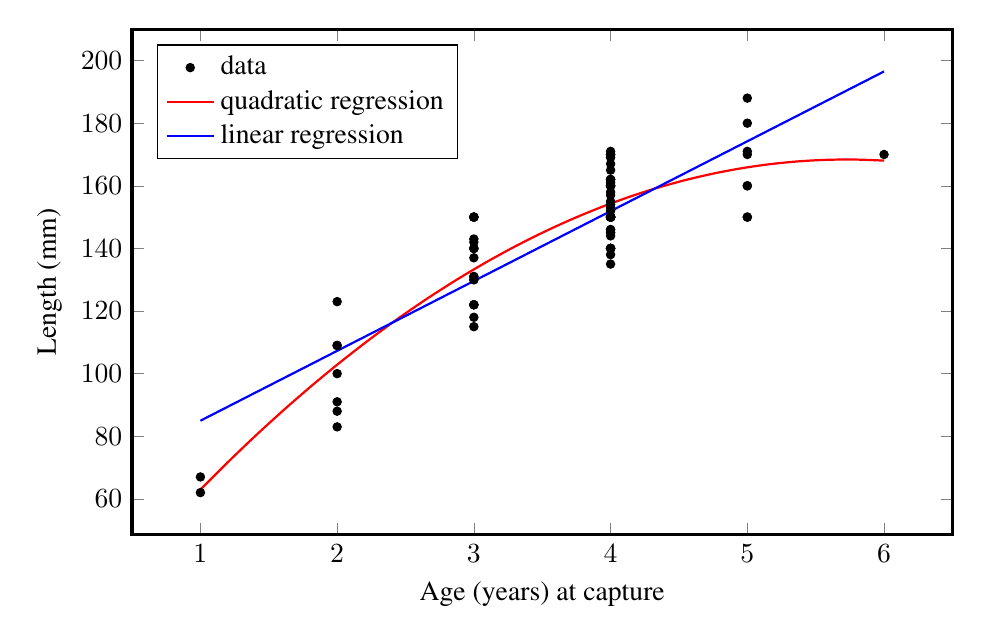
\begin{tikzpicture}
\tikzset{%%
  every mark/.append style={scale=1.0},%%
  scale=1.0%%
}
\pgfplotsset{%%
  every axis/.append style={font=\normalsize}%%
}
%%
\begin{axis}[%%
  axis line style=very thick,%%
  dotStyle/.style={mark size=1.5,black,mark color=black,mark=*,only marks},%%
  enlargelimits=true,%%
  height=8cm,%%
  legend cell align=left,%%
  legend pos=north west,%%
  plotStyle/.style={%%
    domain=1:6,%%
    mark=none,%%
    smooth,%%
    thick%%
  },%%
  width=12cm,%%
  %% x axis
  xlabel={\normalsize Age~(years) at capture},%%
  %% y axis
  ylabel={\normalsize Length~(mm)}%%
]
%%
%%
\addplot[dotStyle] coordinates {
  (1, 67)
  (1, 62)
  (2, 109)
  (2, 83)
  (2, 91)
  (2, 88)
  (2, 123)
  (2, 100)
  (2, 109)
  (3, 137)
  (3, 131)
  (3, 122)
  (3, 122)
  (3, 118)
  (3, 115)
  (3, 131)
  (3, 143)
  (3, 142)
  (3, 122)
  (3, 140)
  (3, 150)
  (3, 140)
  (3, 150)
  (3, 150)
  (3, 140)
  (3, 150)
  (3, 130)
  (3, 130)
  (4, 138)
  (4, 135)
  (4, 146)
  (4, 146)
  (4, 145)
  (4, 145)
  (4, 144)
  (4, 140)
  (4, 150)
  (4, 152)
  (4, 157)
  (4, 155)
  (4, 153)
  (4, 154)
  (4, 158)
  (4, 162)
  (4, 161)
  (4, 162)
  (4, 165)
  (4, 171)
  (4, 162)
  (4, 169)
  (4, 167)
  (4, 150)
  (4, 170)
  (4, 140)
  (4, 140)
  (4, 150)
  (4, 150)
  (4, 150)
  (4, 160)
  (4, 150)
  (4, 150)
  (4, 150)
  (4, 150)
  (4, 140)
  (4, 160)
  (4, 170)
  (4, 160)
  (4, 160)
  (4, 170)
  (5, 171)
  (5, 188)
  (5, 170)
  (5, 150)
  (5, 150)
  (5, 160)
  (5, 160)
  (5, 180)
  (6, 170)
};
\addlegendentry{data}
%%
%%
\addplot+ [plotStyle,red]
{-4.7187*x^2 + 54.0493*x + 13.6224};
\addlegendentry{quadratic regression}
%%
%%
\addplot+ [plotStyle,blue]
{22.3123*x + 62.6490};
\addlegendentry{linear regression}
\end{axis}
\end{tikzpicture}

\end{document}
